\chapter{Command and Control}

\begin{center}
    \makebox[\textwidth]{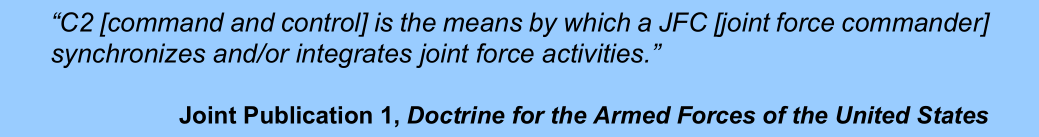
\includegraphics[width=\paperwidth]{quote2.png}}
\end{center}

\section{Introduction}

\e
	\item Le \gls{cas} requiert une structure \gls{cc} intégrée, flexible, et qui réagit rapidement.
	
	\item Le \gls{jfc} exerce son \gls{opcon} via les commandants des différentes composantes, le \gls{jfacc} pour le \gls{cas} (généralement).
\ed

\section{Le CAS en opération mixte}

\e
	\item Il n'y a pas de structure \gls{cc} pré-établie unique pour les opérations de \gls{cc}.
	\itemt{\gls{awacs}}{
	L'\gls{awacs} fournit les informations de transit, et le contrôle et la surveillance radar pour les appareils se déplaçant entre leur base et leur zone d'opération. L'\gls{awacs} soutient les opérations de \gls{cas} en servant de relais entre les appareils de \gls{cas} et l'\gls{opcon}. L'\gls{awacs} à l'autorité pour établir le \gls{stack} des appareils.}
\ed

\section{Systèmes de communications}

\e
	\itemt{Contrôle et flexibilité}{
	Les missions \gls{cas} demandent un contrôle rapproché, rendu possible par des communications efficaces. Les communications doivent être flexibles et rapides pour s'assurer que le lien entre les unités au sol et les appareils qui les soutiennent est maintenu.}
	\item Tous les participants au \gls{cas} doivent connaître les call-signs et fréquences utilisés par les agences de contrôle et les \gls{jtac} qu'ils devront contacter.
\ed